



\section{Categorias de Arquiteturas de Computadores}
	\subsection{Introdução}
%\frame{
%    \Huge \color{blue} \bf  \centering Introdução
%}
\begin{frame}{Introdução}
	\begin{itemize}
	\item Taxonomia de Flynn descreve \textbf{categorias} de \textbf{arquiteturas de sistema de computadores}:
	\end{itemize}

	\begin{figure}[h]
		\centering
		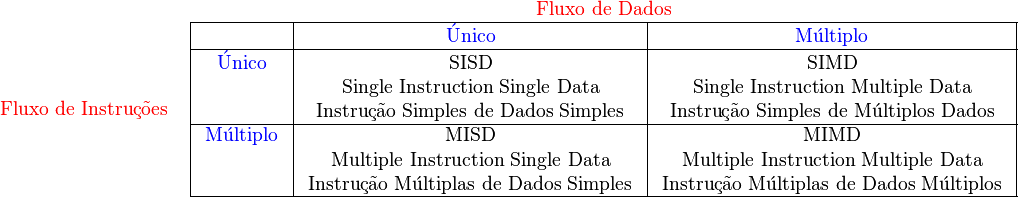
\includegraphics[width=1\textwidth]{img/tobias/taxonomia.png}
		\caption{Taxonomia de Flynn.}
		\label{fig:taxonomia}
	\end{figure}

\end{frame}

%\begin{frame}
%	\begin{itemize}
%		\item Nesta categorização encontra-se a diferenciação de
%		\begin{itemize}
%			\item Multicomputadores e Multiprocessadores; 
%			\item Memória Compartilhada e Memória Distribuída.
%		\end{itemize}
%		
%		\item Os tópicos abordados nesta apresentação serão:
%		\begin{itemize}
%			\item Single Instruction - Simple Data(SISD);
%			\item Single Instruction - Multiple Data(SIMD);
%			\item Multiple Instruction - Multiple Data(MIMD);
%			\item Memória Compartilhada;
%			\item Memória Distribuída;
%			\item ccNUMA;
%			\item Cluster;
%			\item Multiple Instruction - Simple Data(MISD);
%		\end{itemize}
%                
%                \bigskip
%                
%		\item Esta é \textit{válida} até os dias atuais.
%	\end{itemize}
%\end{frame}







%\frame{
%    \huge \color{blue}  \centering {\bf Single} Instruction - {\bf Single} Data (SISD) \\ e \\ {\bf Single} Instruction - {\bf Multiple} Data (SIMD)
%}
%\begin{frame}
%	\begin{itemize}
%		\item \textbf{SISD (Single Instruction - Single Data)}:
%		\begin{itemize}
%    		\item Executa apenas \textbf{1 instrução por ciclo de clock};
%    		\item Apenas 1 conjunto de dados ou operando;
%			\item Utiliza-se \textit{\bf pipeline} para melhorar eficiência;
%			\item Possui problemas com {\it branchs}.
%		\end{itemize}
%		\item \textbf{SIMD (Single Instruction - Multiple Data)}:
%		\begin{itemize}
%			\item Com a \textbf{computação numérica}, permitiu-se o uso de vários conjuntos de dados \textbf{com o mesmo operador}.
%			\item A arquitetura que executa uma instrução para vários dados é chamada de \textbf{vetorial} (Computadores 
%			Vetoriais) e de forma {\it parecida} \textbf{pipeline escalar}.
%			\item Entretanto, eles trabalham com \textbf{vetores de dados} processados em \textbf{1 ciclo}:
%			\begin{itemize}
%				\item Um computador vetorial com \textit{64 elemento} de vetores pode gerar até {\it 64 resultados por ciclo};
%				\item Diferentemente do processador escalar que necessitaria de exatos de 64 ciclos prévios;
%			\end{itemize}
%	
%				\bigskip
%
%		\end{itemize}
%		%\item Categorizações SISD e SIMD {\it não} fazem parte do conceito de multiprocessadores/multicores {\it nem} necessitam de compartilhamento de memória.
%	\end{itemize}
%\end{frame}
%\frame{
%    \Huge \color{blue} \bf  \centering Single Instruction - Single Data (SISD)
%}
%\begin{frame}{Single Instruction - Single Data (SISD)}
%	\begin{itemize}
%		\item Arquitetura que possui tipo de execução mais simples:
%		\begin{itemize}
%    		\item Executa apenas 1 instrução por ciclo de clock.
%    		\item Apenas 1 conjunto de dados ou operando.
%		\end{itemize}
%
%		\item Também chamado de \textbf{Computação Escalar}. 
%	\end{itemize}
%
%	\begin{figure}[h]
%		\centering
%		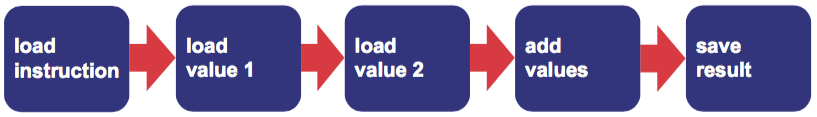
\includegraphics[width=0.9\textwidth]{img/tobias/sisd1.png}
%		\caption{Soma de 2 operando.}
%		\label{fig:sisd1}
%	\end{figure}
%
%	\begin{itemize}
%		\item \textbf{Problema:} Para adicionar 5 pares de números, necessita de $n * 5$ clocks.
%		%\item Cada um das etapas mostradas na Figura~\ref{fig:sisd1} possui sub-etapas piorando a execução da máquina.
%	\end{itemize}
%
%\end{frame}
%
%
%\begin{frame}{Single Instruction - Single Data (SISD)}
%    \begin{itemize}
%		\item Então, pra tornar mais eficiente, utiliza-se \textbf{pipelining}.
%%		\item Por exemplo,
%%		\begin{itemize}
%%			\item  Se existe \textbf{unidade funcional} para os 5 passos da soma, então gasta-se 5 ciclos.
%%			\begin{itemize}
%%    		    \item Se todas as unidades estiverem ocupadas, existirá um resultado a cada ciclo. 
%%			\end{itemize}
%%
%%    		\item Para a soma de $N$ números teríamos somente $(n - 1) + 5$ ciclos de clock.
%%		\end{itemize}
%%
%%	\end{itemize}
%%
%%\end{frame}
%%
%%
%%\begin{frame}{Single Instruction - Single Data (SISD)}
%%    \begin{itemize}
%		\item Instruções normalmente possuem mais de 5 passos implicando em pipelines longos nos processadores reais:
%		\begin{itemize}
%			\item Implicam também em frequência de clock alta.
%		\end{itemize}
%
%		\item Entretanto, longos pipeline possuem problemas com desvios:
%		\begin{itemize}
%			%\item Deve ser \textbf{esvaziado} e \textbf{preenchido} novamente;
%			%\item Há um número de ciclos (igual ao tamanho do pipeline) para que possa ficar eficiente novamente.
%
%			\item Deseja-se que o \textbf{número de desvios} seja \textbf{pequeno}; ou 
%			\item \textbf{Reposicionamento} dos desvios de forma inteligente:
%			\begin{itemize}
%			    \item \textit{Branch prediction}.
%			\end{itemize}
%
%		\end{itemize}
%
%%	\end{itemize}
%%
%%\end{frame}
%%
%%
%%\begin{frame}{Single Instruction - Single Data (SISD)}
%%    \begin{itemize}
%		\item Processadores podem ter um \textbf{desempenho superior} utilizando combinações de \textbf{vários pipelines} (Processadores Superescalares):
%		\begin{itemize}
%			\item \textbf{Cálculos Lógico/Aritiméticos} (ALU) são separados de \textbf{Pontos Flutuantes} (FPU).
%			\item Normalmente, FPU é dividido em uma unidade para adição e outra para multiplicação.
%			\begin{itemize}
%			    \item Além de unidades de divisão e computação de raiz quadrada.
%			\end{itemize}
%
%		\end{itemize}
%
%		%\item Hoje, o ganho deste tipo de arquitetura está nos \textbf{vários pipelines} no qual podem ser usados \textbf{ao mesmo tempo}.
%	\end{itemize}
%
%\end{frame}
%
%
%
%
%
%
%
%
%\frame{
%    \Huge \color{blue} \bf  \centering Single Instruction - Multiple Data (SIMD)
%}
%
%\begin{frame}{Single Instruction - Multiple Data (SIMD)}
%	\begin{itemize}
%		\item Com a \textbf{computação numérica}, permitiu-se o uso de vários conjuntos de dados \textbf{com o mesmo operador}.
%		\item A arquitetura que executa uma instrução para vários dados é chamada de \textbf{vetorial} (Computadores Vetoriais) e de forma parecida \textbf{pipeline escalar}.
%		\item Entretanto, eles trabalham com \textbf{vetores de dados} processados em \textbf{1 ciclo}:
%		\begin{itemize}
%			\item Um computador vetorial com 64 elemento de vetores pode gerar até 64 resultados por ciclo;
%			\item Diferentemente do processador escalar que precisa de 64 ciclos prévios;
%		\end{itemize}
%
%	\end{itemize}
%
%	
%\end{frame}
%
%
%\begin{frame}{Single Instruction - Multiple Data (SIMD)}
%	\begin{itemize}
%		\item Pra utilizar todo seu desempenho de processamento, os cálculos por ele executado \textbf{também devem ser 
%		naturalmente vetoriais} e utilizar \textbf{todos os recursos disponíveis}.
%%		\item Usados no âmbito de computação com alta performance:
%%		\begin{itemize}
%%			\item Permite alta performance com baixa frequência de clock.
%%		\end{itemize}
%
%%	\end{itemize}
%%
%%\end{frame}
%%
%%
%%\begin{frame}{Single Instruction - Multiple Data (SIMD)}
%%	\begin{itemize}
%%		\item Estão desaparecendo lentamente com o passar dos anos:
%%		\begin{itemize}
%			\item São \textbf{complexos} e \textbf{caros} e não suportam bem \textbf{problemas não-vetoriais}.
%		    \item Computadores escalares são baratos e possuem alta frequência de clock.
%%		\end{itemize}
%
%%		\item Computadores vetoriais não foram disseminados totalmente:
%%		\begin{itemize}
%%			\item Com o Pentium III, a Intel introduziu o SSE (Streaming SIMD Extension) que possuía um conjunto de instruções vetoriais;
%%			\item Logo em seguida:
%%			\begin{itemize}
%%			    \item SSE2 com o Pentium IV;
%%			    \item SSE3 com o Pentium IV Pescott.
%%			\end{itemize}
%%
%%		\end{itemize}
%
%	\end{itemize}
%
%\end{frame}






	\subsection{Memória Compartilhada, Distribuída e suas Combinações}
%\frame{
%    \Huge \color{blue}  \centering {\bf Multiple} Instruction - \\ {\bf Multiple} Data (MIMD)
%}
\begin{frame}{Multiple Instruction - Multiple Data (MIMD)}
	\begin{itemize}
		%\item Até então foi considerado operações que executam em \textbf{1 ciclo de clock}.
		%\item Isso aplica-se a todos os computadores que possui \textbf{1 processador de 1 core}.
		\item Arquiteturas com vários cores ou vários processadores \textbf{independente da classe (escalar/vetor)}, são declaradas MIMD.
		\item Todos os processadores de alta performance pertence a essa categoria.

				\bigskip

		\item Pode ser subdividida de acordo com a arquitetura de memória:
		\begin{enumerate}
			\item Memória Compartilhada;
			\item Memória Distribuída;
			\item Combinações.
		\end{enumerate}

	\end{itemize}

\end{frame}








\begin{frame}{Memória Compartilhada - SM-MIMD}
	\begin{itemize}
		\item MIMD com memória compartilhada (SM-MIMD) são processadores que são conectados \textbf{num barramento comum de memória RAM}.
		\item Também pode ser nomeado como Multiprocessamento Simétrico
		\begin{itemize}
			\item \textbf{Processadores devem ser idênticos} e possuem \textbf{igual acesso à memória};
			%\item Podem ser encontrados em PC e pequenos servidores.
		\end{itemize}

	\end{itemize}

\end{frame}


\begin{frame}{Memória Compartilhada - SM-MIMD}
    \begin{figure}[h]
    	\centering
    	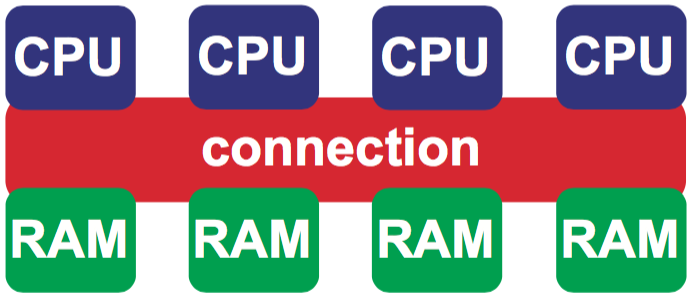
\includegraphics[width=0.95\textwidth]{img/tobias/sm-mimd.png}
    	\caption{\textbf{Modelo} MIMD com compartilhamento de memória.}
    	\label{fig:sm-mimd}
    \end{figure}

\end{frame}


\begin{frame}{Memória Compartilhada - SM-MIMD}
    \begin{figure}[h]
    	\centering
    	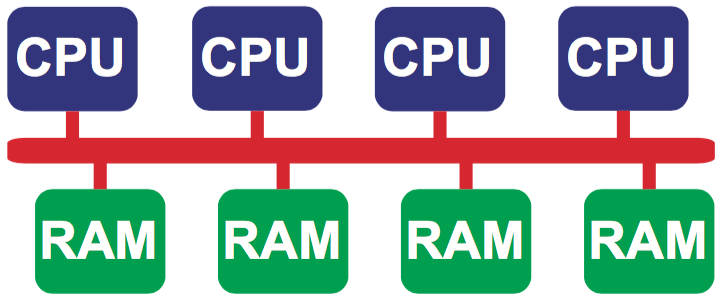
\includegraphics[width=1\textwidth]{img/tobias/sm-mimd2.png}
    	\caption{MIMD com compartilhamento de memória por meio de {\bf 1 único barramento}.}
    	\label{fig:sm-mimd2}
    \end{figure}

\end{frame}


\begin{frame}{Memória Compartilhada - SM-MIMD}
	\begin{itemize}
		\item \textbf{Vantagem:}
		\begin{itemize}
	    	\item Expansibilidade.
		\end{itemize}

			\bigskip

		\item \textbf{Desvantagem:}
		\begin{itemize}
		    \item Todos devem compartilhar a mesma largura de banda, mesmo acessando diferentes módulos de memória.
		\end{itemize}

		\item Com isso, a conexão entre processador e memória torna-se item essencial na eficiência.
	\end{itemize}

\end{frame}


\begin{frame}{Memória Compartilhada - SM-MIMD}
    \begin{figure}[h]
    	\centering
    	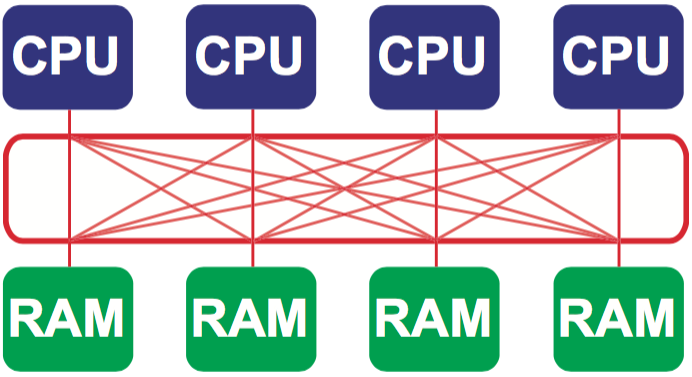
\includegraphics[width=1\textwidth]{img/tobias/sm-mimd3.png}
    	\caption{MIMD com compartilhamento de memória por meio de um {\bf comutador}.}
    	\label{fig:sm-mimd3}
    \end{figure}

\end{frame}


\begin{frame}{Memória Compartilhada - SM-MIMD}
	\begin{itemize}

		\item Computadores de alta performance e \textit{workstations}.

						\bigskip
		\item \textbf{Vantagem:}
		\begin{itemize}
		    \item Todos os processadores podem comunicar com as memórias tornando o \textit{software} fácil para desenvolvimento e eficiente para o uso.
		\end{itemize}

			\bigskip

		\item \textbf{Desvantagem:}
		\begin{itemize}
			\item Possuem um alto \textbf{grau de complexabilidade} quando muitas conexões devem ser feitas.
			\begin{itemize}
			    \item Grafo Bipartido Completo: Para $m + n$ vértices, existe $m*n$ arestas.
			    \item Utiliza-se uma variante dessa com comutadores multi-estágios para reduzir este problema.
			\end{itemize}
		\end{itemize}

	\end{itemize}

\end{frame}








\begin{frame}{Memória Distribuída - DM-MIMD}
	\begin{itemize}
		%\item Ao utilizar memória compartilhada, torna-se complicado a tarefa de acrescentar arbitrariamente o número de memória e processadores.
		%\item E sobre este problema, existe outro meio no qual utiliza-se \textbf{Memória Distribuída} (DM-MIMD).
		%\begin{itemize}
			\item Cada processador \textbf{possui sua memória local} e são \textbf{conectados entre si}.
			\item As exigências nesta rede são mais baixa
			\begin{itemize}
			    \item Entretanto a troca de informação é \textbf{mais lenta}.
			\end{itemize}
		%\end{itemize}

	\end{itemize}

\end{frame}


\begin{frame}{Memória Distribuída - DM-MIMD}
    \begin{figure}[h]
    	\centering
    	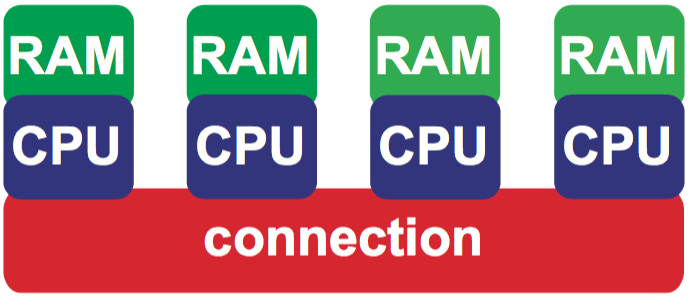
\includegraphics[width=1\textwidth]{img/tobias/dm-mimd.png}
    	\caption{MIMD com distribuição de memória.}
    	\label{fig:dm-mimd}
    \end{figure}

\end{frame}


%\begin{frame}
%    \begin{figure}[h]
%    	\centering
%    	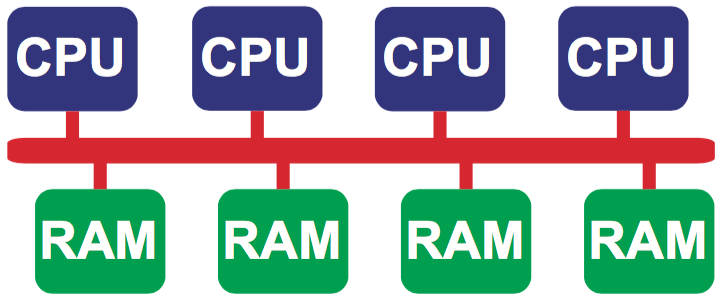
\includegraphics[width=0.6\textwidth]{img/tobias/sm-mimd2.png}
%    	\caption{Compartilhamento de memória por meio de {\bf 1 único barramento}.}
%    	\label{fig:sm-mimd2}
%    \end{figure}
%
%    		\bigskip
%
%    \begin{figure}[h]
%    	\centering
%    	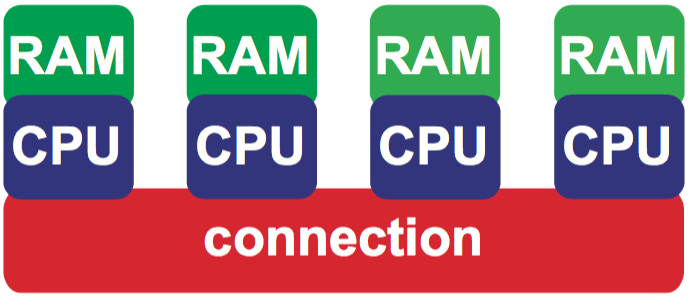
\includegraphics[width=0.6\textwidth]{img/tobias/dm-mimd.png}
%    	\caption{Distribuição de memória.}
%    	\label{fig:dm-mimd}
%    \end{figure}
%
%\end{frame}

\begin{frame}{Memória Distribuída - DM-MIMD}
	\begin{itemize}
		%\item Necessita de mais esforço na \textbf{programação} do que no \textbf{sistema de memória compartilhada}.
		\item Podem ser expandidas facilmente e utilizar modelos de processador/memória diferentes.
		\item O uso de milhares de processadores \textbf{não-comuns} são chamados de \textbf{Processamento Massivamente Paralelo}.
		\item Os problemas são divididos em \textit{subproblemas} no qual necessitam de pouca comunicação:
		\begin{enumerate}
			\item Processador usa sua \textbf{própria memória};
			\item Se deseja algum dado de outra memória, ele é \textbf{copiado};
			\item A \textbf{requisição de informação} deve ser evitada\footnote{Utiliza-se mensagens.} sendo o motivo da comunicação entre eles é \textbf{lenta}.
		\end{enumerate}

	\end{itemize}

\end{frame}








\begin{frame}{ccNUMA}
	\begin{itemize}
		\item Problemas até então:
			\begin{itemize}
				\item {\bf SM-MIMD:} tamanho limitado.
				\item {\bf DM-MIMD:} árduo sistema de comunicação.
			\end{itemize}

				\bigskip

		\item ccNUMA\footnote{\textit{cache coherent Non-Uniform Memory Access}, cache de acesso coerente à memória não uniforme.} é uma arquitetura variante que consiste em vários processadores de Memória Compartilhada.
		\item Consiste numa arquitetura que possui \textbf{caches nos processadores} para que {\bf reduza o acesso de dados remotos}.

		\item Possui além do acesso {\bf homogêneo}, o {\bf heterogêneo}  à memória
		\begin{itemize}
			\item Pois cada processador pode ter uma memória local além da compartilhada.
		\end{itemize}
		\item São conectados entre si criando uma rede de comunicação rápida utilizando um {\bf comutador}.
	\end{itemize}

\end{frame}


\begin{frame}
    \begin{figure}[h]
    	\centering
    	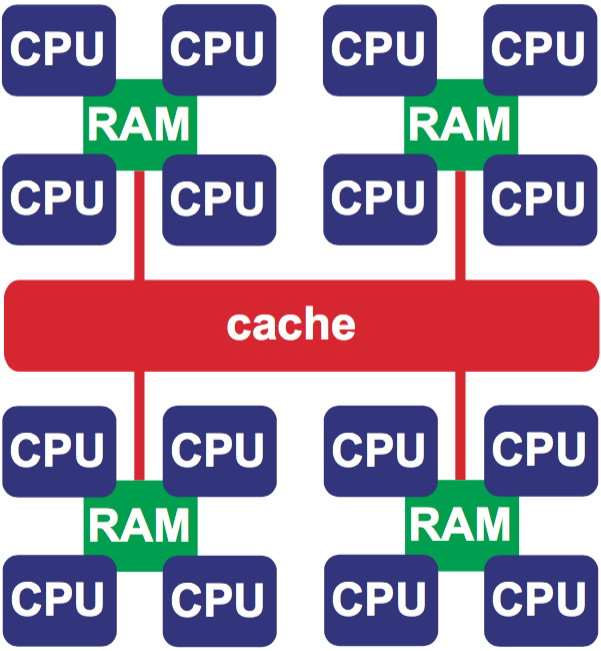
\includegraphics[width=0.6\textwidth]{img/tobias/ccnuma.png}
    	\caption{Arquitetura Paralela ccNUMA heterogênea.}
    	\label{fig:ccnuma}
    \end{figure}
\end{frame}



%\begin{frame}
%    \begin{multicols}{2}
%	
%	    \begin{figure}[h]
%	    	\centering
%	    	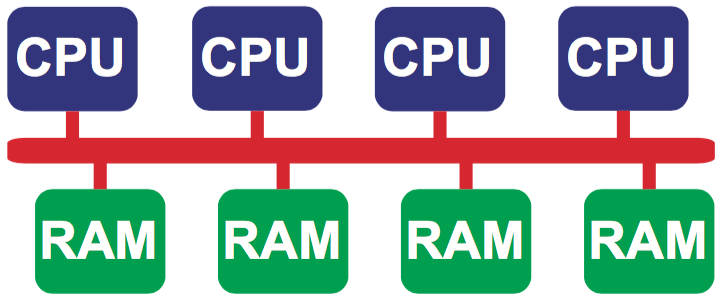
\includegraphics[width=0.42\textwidth]{img/tobias/sm-mimd2.png}
%	    	\caption{Compartilhamento de memória por meio de {\bf 1 único barramento}.}
%	    	\label{fig:sm-mimd2}
%	    \end{figure}
%
%	    \begin{figure}[h]
%	    	\centering
%	    	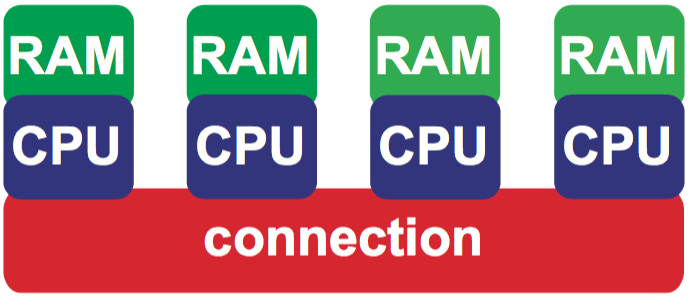
\includegraphics[width=0.42\textwidth]{img/tobias/dm-mimd.png}
%	    	\caption{Distribuição de memória.}
%	    	\label{fig:dm-mimd}
%	    \end{figure}
%
%	\columnbreak
%
%	    \begin{figure}[h]
%	    	\centering
%	    	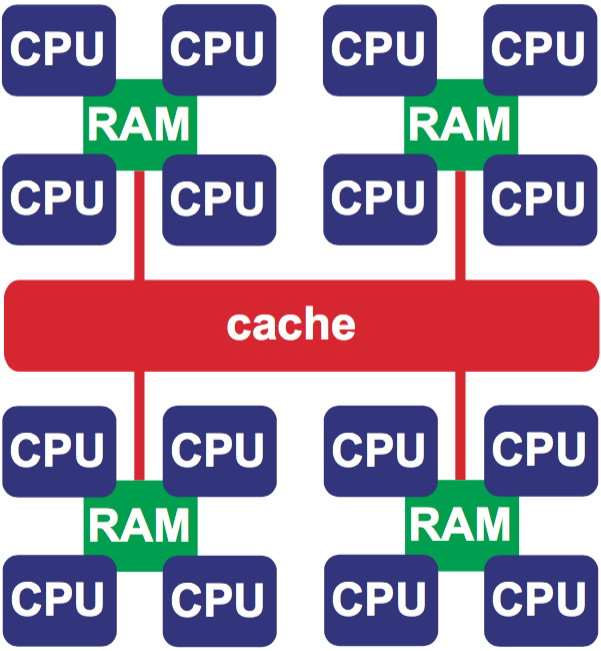
\includegraphics[width=0.42\textwidth]{img/tobias/ccnuma.png}
%	    	\caption{Arquitetura Paralela ccNUMA.}
%	    	\label{fig:ccnuma}
%	    \end{figure}
%
%    \end{multicols}
%
%\end{frame}


%\begin{frame}{ccNUMA}
%    \begin{itemize}
%		\item São conectados entre si criando uma rede de comunicação rápida utilizando um {\bf comutador}.
		
%		    \bigskip
		    
%		\item É fácil utilizar tal como o Memória Compartilhada: 
%		\begin{itemize}
%		    \item Com a vantagem de ser facilmente expansível.
%		\end{itemize}

%		\item Para garantir o desempenho ideal
%		\begin{itemize} 
%			\item Priorizar o uso da {\bf memória local} e não a dos outros módulos.
%		\end{itemize}
%		\item {\bf Módulos} podem ser {\it acoplados/conectados} para obter um sistema maior.	
%	\end{itemize}

%\end{frame}







\begin{frame}{Cluster}
	\begin{itemize}
		\item Clusters são uma forma \textbf{popular} de computação de alta performance.
		\item Consistem em \textbf{vários computadores baratos} conectados entre si.
		\item Conhecidos como \textbf{Rede de \textit{Workstations}} (NOW) e como produto final um Sistema Híbrido
		\begin{itemize}
			\item Os \textbf{nós} teriam \textbf{sistemas de memória compartilhada} formados por \textbf{sistema de memória distribuída}.
		\end{itemize}
	
	\end{itemize}

\end{frame}


\begin{frame}{Cluster}
    \begin{figure}[h]
    	\centering
    	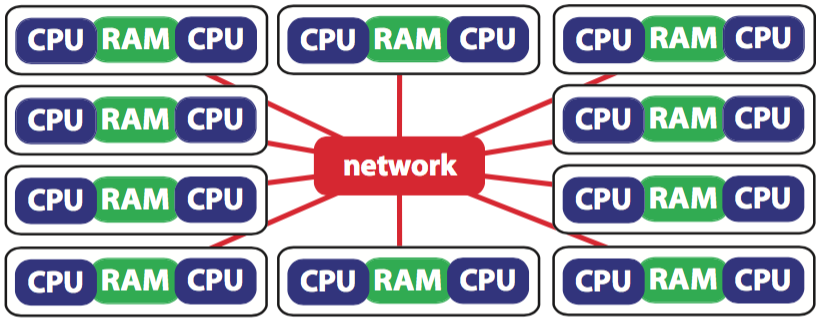
\includegraphics[width=1\textwidth]{img/tobias/cluster.png}
    	\caption{Arquitetura Paralela Cluster.}
    	\label{fig:ccnuma}
    \end{figure}

\end{frame}


\begin{frame}{Cluster}
    \begin{itemize}
%		\item Essa rede distribuída é feita por {\bf redes alta vazão} podendo utilizar comunicações \textbf{Myrinet} ou \textbf{Infiniband}.
%		\begin{itemize}
%			\item \textbf{Gigabit Ethernet} tem alta vazão mas com \textbf{alta latência} no envio dos pacotes.
%			\item Enquanto Gigabit Ethernet possui cerca de $100\mu s$ em latência, Myrinet possui $10 - 20 \mu s$.
%		\end{itemize}
%
%		\item Não é fácil utilizar todo seu poder de processamento:
%		\begin{itemize}
%			\item A comunicação entre nós é lenta pois a comunicação distribuída é naturalmente lenta.
%			%\item Os nós geralmente possui limites de memória\footnote{Arquitetura 32-bit só endereça 4GB e x86-64 possuem 
%			%limitados slots de memória, entre outros possíveis problemas.}.
%		\end{itemize}
%
%%	\end{itemize}
%%
%%\end{frame}
%%
%%
%%\begin{frame}{Cluster}
%%    \begin{itemize}
		\item \textbf{Vantagens:}
		\begin{itemize}
			\item Bem-suscetível para problemas de \textbf{alto nível de paralelismo};
			\item Sua modularidade permite \textbf{modificações} de forma facilitada. 
		\end{itemize}

			\bigskip

		\item Outro tipo de arquitetura é nomeada \textbf{Grid}.
		\begin{itemize}
			\item São sistemas no qual pode utilizar computadores com arquiteturas \textbf{totalmente diferentes};
			\item São espalhados pelo mundo e conectados entre si;
			%\item Podem utilizar a internet como meio de comunicação;
			\item Possuem um alto grau de processamento computacional.
		\end{itemize}

	\end{itemize}

\end{frame}








%\frame{
%    \Huge \color{blue} \bf  \centering Multiple Instruction - Single Data (MISD)
%}
%
%\begin{frame}{Multiple Instruction - Single Data (MISD)}
%	\begin{itemize}
%		\item Não pode ser feita nem pratica ou teoricamente de forma \textbf{sensata}.
%		
%				\bigskip
%		
%		\begin{block}{Openshaw (1999)}
%		    {\it ``Descobrimos que é difícil calcular o porquê você iria fazer `isso', a menos que você seja um cientista da 
%		    computação interessado em computação estranha. É um sistema altamente especializado e restrito e até muitas vezes 
%		    impraticável, pra não dizer inútil como base para uma máquina de uso geral''.}
%		\end{block}
%		
%	\end{itemize}
%
%\end{frame}





\subsection{Multicomputadores e Multiprocessadores}
\begin{frame}{Multicomputadores e Multiprocessadores}
	\begin{multicols}{2}
	
		{\bf Multiprocessador:}
		\begin{itemize}
			\item Existe somente uma memória compartilhada onde é acessada por meio de comandos de (Load e Store).
			\item Não podem ser ampliados facilmente.
			\item UMA e NUMA.
		\end{itemize}
	\columnbreak
		{\bf Multicomputador:}
		\begin{itemize}
			\item Cada processador tem sua memória privada (Memória distribuída).
			\item Utilizam Send e Receive (não Load e Store).
			\item Exemplo:
			\begin{itemize}
				\item Computadores Maciçamente Paralelos\footnote{DM-MIMD não-comuns.};
				\item Clusters\footnote{Centrados e Descentralizados.}.
			\end{itemize}
		\end{itemize}
	            
	\end{multicols}
\end{frame}